\documentclass{article}
\usepackage[utf8]{inputenc}

\usepackage[paperwidth=8.5in, paperheight=11in, top=1in, bottom=.5in, left=.5in, right=.5in]{geometry}
\usepackage{fancyhdr, graphicx,tikz,amsmath,multicol,paracol}
\usepackage[inline]{enumitem}


\pagestyle{fancy}
\lhead{\large{\textbf{Module 6: Trigonometric Functions (TR) - Readiness Assurance Test}}}
\chead{}
\rhead{}
\lfoot{}
\cfoot{}
%\rfoot{\thepage/\pageref{LastPage} }
\setlength{\headheight}{14pt} %added in bc warning

%%% LIST ANSWER KEY HERE

% 1 B
% 2 C
% 3 D
% 4 A
% 5 B
% 6 C
% 7 D
% 8 A
% 9 C
% 10 A


\begin{document}


\begin{enumerate}


% Determine the circumference of a circle given the diameter.

\item A bicycle wheel has a diameter of $26$ inches. What is the circumference of the bicycle wheel? Write your answer in terms of $\pi$.

  \begin{enumerate}
  \begin{multicols}{4}
  \item 13$\pi$   
  \item 26$\pi$ %correct
  \item 169$\pi$
  \item 676$\pi$
  \end{multicols}
  \end{enumerate}

% Determine the quadrant of a point.

\item Which ordered pair locates a point in Quadrant II?

  \begin{enumerate}
  \begin{multicols}{4}
  \item $(-4, -1)$  
  \item $(4, 1)$
  \item $(-4, 1)$ %correct 
  \item $(4,-1)$
  \end{multicols}
  \end{enumerate}

% Determine the measure of an angle of a triangle.

\item In triangle $ABC$, the measure of angle $A$ is $104^{\circ}$ and the measure of angle $C$ is $32^{\circ}$. What is the measure of angle $B$?

  \begin{enumerate}
  \begin{multicols}{4}
  \item $136^{\circ}$ 
  \item $76^{\circ}$
  \item $148^{\circ}$ 
  \item $44^{\circ}$ %correct
  \end{multicols}
  \end{enumerate}

% Use the Pythagorean Theorem to find side lengths of right triangles AND Simplify square roots of positive numbers. This was in another RAT, but I thought it would be a good fit here too.

\item A right triangle has one leg of length $7$ inches and its hypotenuse is $15$ inches. What is the length of the other leg of the triangle? Simplify your answer.

        \begin{enumerate}
        \begin{multicols}{4}
          
          \item $\sqrt{176}$ inches %not simplified
          \item $\sqrt{274}$ inches %treated 7 & 15 both as legs
          \item $4\sqrt{11}$ inches %correct
          \item $2\sqrt{44}$
        \end{multicols}
        \end{enumerate}

% Determine a point on the coordinate plane.

\item A point that lies on the $x$-axis between quadrants I and IV could have the following for the $x$- and $y$-coordinates:

        \begin{enumerate}
        \begin{multicols}{4}
          
          \item $(0,7)$
          \item $(7,0)$ %correct
          \item $(0,-7)$
          \item $(-7,0)$
        \end{multicols}
        \end{enumerate}

% Use the Pythagorean Theorem to find the distance between two points.

\item Use the Pythagorean Theorem to find the distance between points $A$ and $B$.
\begin{center}
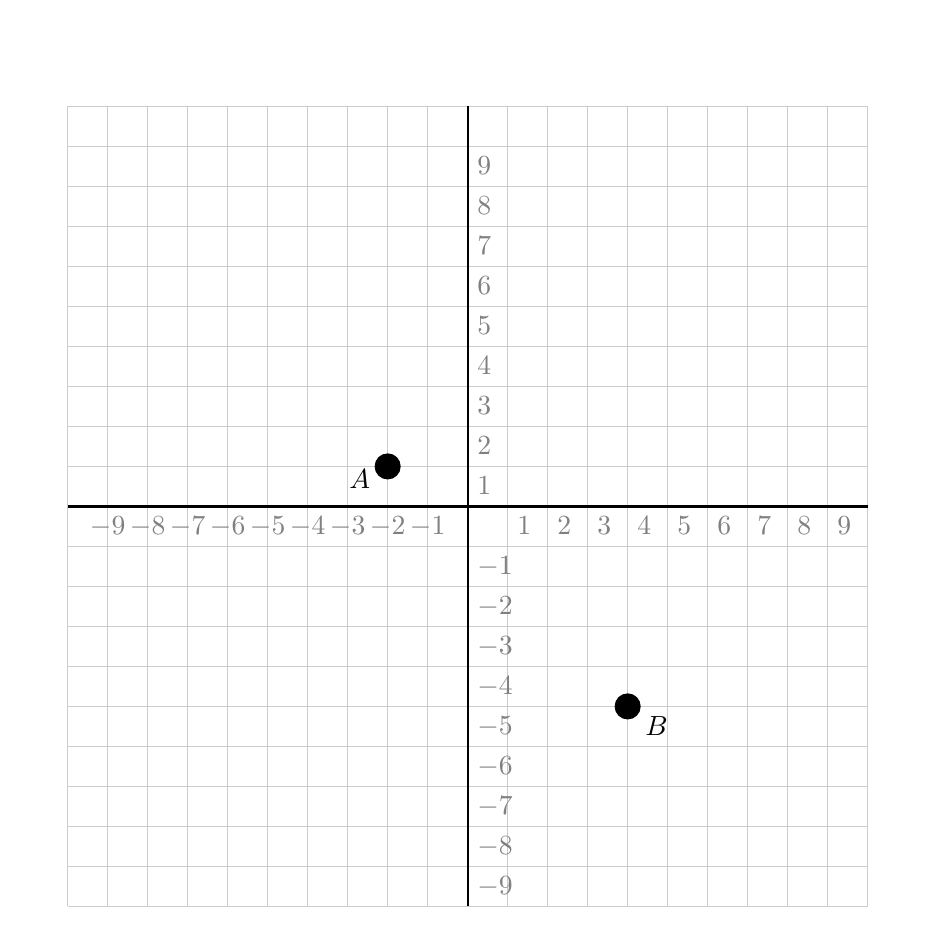
\begin{tikzpicture}[x=0.2in,y=0.2in]
\fill[white] (-11,-11) rectangle (11,11);
\draw[black!20,step=1] (-10,-10) grid (10,10);
\draw[thick] (0,-10) -- (0,10);
\draw[thick] (-10,0) -- (10,0);
\node[circle,fill] at (-2,1) {};
\node[anchor=south west] at (-3.2,0.2) {$A$};
\node[circle,fill] at (4,-5) {};
\node[anchor=north west] at (4.2,-5) {$B$};
\foreach \i in {-9,...,-1}
  {\node[anchor=north,thin,gray] at (\i,0) {$\i$};
  \node[anchor=north west,thin,gray] at (0,\i) {$\i$};}
\foreach \i in {1,...,9}
  {\node[anchor=north west,thin,gray] at (\i,0) {$\i$};
  \node[anchor=north west,thin,gray] at (0,\i) {$\i$};}
\end{tikzpicture}
\end{center}

\begin{enumerate}
        \begin{multicols}{4}
          
          \item $2\sqrt{3}$ 
          \item $6$
          \item $6\sqrt{2}$ %correct
          \item $2\sqrt{6}$
        \end{multicols}
        \end{enumerate}

\pagebreak

% Determine the measure of a third angle of a right triangle.

\item A right triangle has an acute angle which measures $40^{\circ}$. What is the measure of the other acute angle?

        \begin{enumerate}
        \begin{multicols}{4}
          
          \item $60^{\circ}$
          \item $40^{\circ}$ 
          \item $90^{\circ}$
          \item $50^{\circ}$ %correct
        \end{multicols}
        \end{enumerate}

\vspace{5pt}
\hspace{-15pt}\textbf{Use the right triangle $ABC$, as shown in the figure below, to answer questions 8-10.}

\begin{center}
    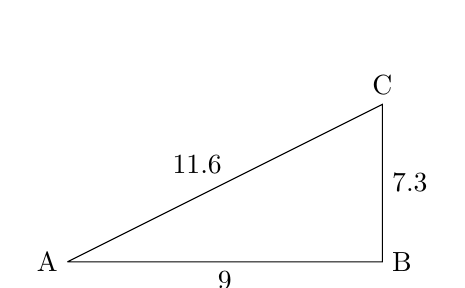
\begin{tikzpicture}
        \coordinate (a) at (0,0);
        \coordinate (b) at (4,0);
        \coordinate (c) at (4,2);
        \draw (a) -- (b)node[midway, below]{\(9\)} -- (c)node[midway,right]{\(7.3\)} -- (a)node[midway,left={1em}, above]{\(11.6\)}; % Triangle.

        \draw (a) node[anchor=east,align=center] {A};
        \draw (b) node[anchor=west,align=center] {B};
        \draw (c) node[anchor=south]{C};
    \end{tikzpicture}
    \end{center}

% Determine the side of a triangle given an image.

\item What is the length of side $a$?

        \begin{enumerate}
        \begin{multicols}{4}
          
          \item $7.3$ %correct
          \item $9$ 
          \item $11.6$
          \item $90$ 
        \end{multicols}
        \end{enumerate}

\item What is the length of the hypotenuse?

        \begin{enumerate}
        \begin{multicols}{4}
          
          \item $7.3$ 
          \item $9$ 
          \item $11.6$ %correct
          \item $90$ 
        \end{multicols}
        \end{enumerate}

\item What is the length of the side that is adjacent to angle $C$?

        \begin{enumerate}
        \begin{multicols}{4}
          
          \item $7.3$ %correct
          \item $9$ 
          \item $11.6$ 
          \item $90$ 
        \end{multicols}
        \end{enumerate}
 
\end{enumerate}


\end{document}